\section{Echte Strategie}

\begin{frame}[c]{Strategie}
    \Large
    Ein Ziel ist das Was. \\
    Gründe sind das Warum. \\
    \pause
    Strategie ist das Wie.
\end{frame}


\subsection{Kernel}


\begin{frame}[c]{Kernel - was ist das}
    \large
    Jede gute Strategie hat eine gemeinsame zugrundeliegende Struktur
\end{frame}


\begin{frame}[c]{Kernel - besteht aus}
    \Large
    \begin{itemize}
        \item Diagnose
            \pause
        \item Eine Leitende Idee
            \pause
        \item Menge Zusammenhängender Aktionen
    \end{itemize}
    % Bsp:
    % - Arzt
    % - Autofahren
\end{frame}


\begin{frame}[c]{Kernel - unerwähnt}
    \begin{itemize}
        \item Visionen
        \item Hierarchien
            \pause
        \item Ziele
        \item Zeitspannen
            \pause
        \item Reichweite
        \item Ideen zur Veränderung
    \end{itemize}
    % Explizit unerwähnt, da nicht teil der Grundstruktur
\end{frame}


\subsection{Diagnose}


\begin{frame}[c]{Kernel - Diagnose}
    \Huge
    Die Große Frage: \\
    \pause
    Was passiert hier eigentlich?
\end{frame}


\begin{frame}[c]{Wirklich die richtige Situation sehen}
    \Huge
    Erinnert ihr euch an Cached Thoughts?
\end{frame}


\begin{frame}[c]{Das Bayes'sche Theorem}
    \Large
    \[
        P(A|X) = \frac{P(X|A) * P(A)}{P(X|A) * P(A) + P(X|\neg A) * P(\neg A)}
    \]
\end{frame}


\begin{frame}[c]{Bayes'sche Theorem: xkcd}
    \begin{multicols}{2}
    \begin{itemize}
        \item[]<1> 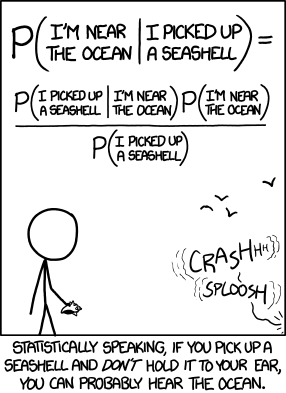
\includegraphics[height=7cm]{strategy/xkcd_seashell.png}
        \item[]<2> 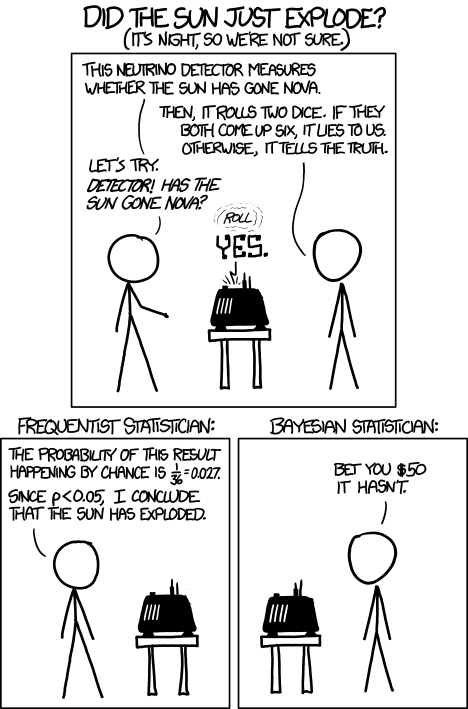
\includegraphics[height=7cm]{strategy/xkcd_frequentists_vs_bayesians.png}
    \end{itemize}
    \end{multicols}
\end{frame}


\begin{frame}[standout]
    Ist es möglich dass es anders ist als es scheint?
    % Notes:
    % Bsp:
    % Kein Event bevorzugen,
    % andere, gleichwahrscheinliche beachten
    % Aha-Moment sonst nicht möglich
    % Genauso: Erkennen der eigentlichen Situation
\end{frame}


\begin{frame}[c]{Diagnose - Beispiel}
    IBM, 1993, es ging Bergab. \\
    Diagnose: Zu groß. \\ \pause
    Neue Diagnose: Zu wenig vernetzt.
\end{frame}


\subsection{Leitidee}


\begin{frame}[c]{Leitidee - Was ist das}
    \Large
    Die grobe richtung, {\em WIE} man weiter vorgeht.
\end{frame}


\begin{frame}[c]{Leitidee - Beispiel}
    \Large
    Kleiner Eckladen
\end{frame}


\subsection{Zusammenhängende Aktionen}


\begin{frame}[c]{Menge Zusammenhängender Aktionen}
    \Huge
    Klingt einfach. Ist es nicht.
    % eigentliche Strategie
\end{frame}


\begin{frame}[c]{Menge Zusammenhängender Aktionen}
    \Huge
    Eigentlicher Teil der Strategie
\end{frame}


\begin{frame}[c]{Zusammenhängende Aktionen}
    \Huge
    Koordinierte Aktionen
\end{frame}


\subsection{Fazit}


\begin{frame}[c]{Kernel}
    \Large
    \begin{itemize}
        \item Diagnose
            \pause
        \item Eine Leitende Idee
            \pause
        \item Menge Zusammenhängender Aktionen
    \end{itemize}
    % Bsp:
    % - Arzt
    % - Autofahren
\end{frame}


\begin{frame}{Kernel - Fazit}
    \large
    Sehr wichtige Grundbausteine, \\
    Sehr vieles wird schiefgehen sollten diese nicht vorhanden sein.
\end{frame}






